\documentclass[11pt]{article}
%---- defitions ----
\def\Author{Andreas Bock\\
Asbj\o rn Thegler\\
Lasse Dessau
}
\def\Title{\bf Principles of Computer Systems Design\\ {\Large Assignment 1}}
% <Add more defitions here>
%-------------------

%---- packages ----
\usepackage[]{amsmath}
\usepackage[english]{babel}
\usepackage[utf8]{inputenc}
\usepackage{graphicx}
\usepackage{moreverb}
\usepackage{hyperref}
\usepackage{color}
\usepackage{listings}
\usepackage{algorithmicx}
\usepackage{algorithm}
\usepackage{algpseudocode}
\usepackage[T1]{fontenc} % font
\usepackage{program}
\usepackage[top=2in, bottom=0.5in, left=1.4in, right=1.4in]{geometry}
%---- settings ----
% Comments
\newcommand{\comm}[2]{{\sf \(\spadesuit\){\bf #1: }{\rm \sf #2}\(\spadesuit\)}}
\newcommand{\mcomm}[2]{\marginpar{\scriptsize \comm{#1}{#2}}}
\newcommand{\ab}[1]{\mcomm{AB}{#1}} % Andreas Bock

\topmargin=-0.9in % start text higher on page
\textheight=695pt
\setlength{\parindent}{0in}
\definecolor{lightgray}{rgb}{0.9,0.9,0.9}
\renewcommand*\rmdefault{ppl} % font
%-------------------

\begin{document}
\title{\Title}
\author{\Author}
\date{\today}
\maketitle

\section*{Question 1: Serializability \& Locking}

\section*{Question 2: Optimistic Concurrency Control}

\section*{Programming Task}

In this section we go through our implementation and how our choice of
concurrency control protocol adheres to the requirements of
\texttt{acertainbookstore.com}.

\subsection*{Implementation}

As stated in the assignment text, the \texttt{synchronized} keyword has
been removed to allow for finer grained concurrency control by using
appropriate locks.
This has been achieved by using a \href{http://docs.oracle.com/javase/6/docs/api/java/util/concurrent/locks/ReentrantReadWriteLock.html}{\texttt{ReentrantReadWriteLock}}  ,
which allows us to declare read and write locks with the desired semantics.

Our concurrency control protocol uses strict two-phase locking (S2PL), a solution which
relies on locks to achieve conflict serializability.
In other words, acquisition of the locks follows the diagram from Marcos'
slides (figure ~\ref{fig:lock}).\\

\begin{figure}[h!]
\begin{center}
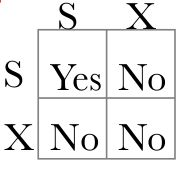
\includegraphics[scale=0.45]{lock.png}
\caption{Locking solution for isolation.}
\label{fig:lock}
\end{center}
\end{figure}

More concretely, this means that methods such as \texttt{getEditorPicks} and
\texttt{getBooks} need only acquire the read lock, while the methods that
need to read \emph{and} write follow the pseudocode described in algorithm
\ref{lst:readwrite}.\\

\begin{algorithm}
\caption{Pseudocode for methods that need to read and write}
\label{lst:readwrite}
\begin{algorithmic}
\Function{readAndWriter}{someParams}\\
\hspace{0.58cm}\Call{acquireReadLock()}{}
\If {requiryIsValid}\\
\hspace{1.16cm}\Call{acquireWriteLock()}{}
    \State $result\gets \Call{doWrite}{someParams}$
\Else
    \State $result\gets Error$
\EndIf\\
\hspace{0.58cm}\Call{unlockAcquired()}{}\\
\hspace{0.58cm}\Return $result$
\EndFunction
\end{algorithmic}
\end{algorithm}

It is clear that the method described in the pseudocode follows S2PL, as
we acquire locks on the fly, and release everything at the end.\\

We can expect higher throughput as we now allow for multiple readers, which
is convenient for a book store where you may have several customers browsing
the wares.

\subsection*{Testing}

We have added the two required tests described in the assignment text, along
with $SOME$ other tests.

\subsubsection*{Test 1}

The assignment text states: "\emph{the clients invoke a fixed number of operations,
configured as a parameter...}". This is not clear to us what is meant by this, as
it seems excessive to create a new class where we translate the parameters (along with
parameters such as \texttt{Set<StockBook>} for \texttt{addBooks}.

We should probably add a \texttt{volatile} keyword to the mapping.

However, we hard-code the 

Otherwise we would have to parse a string and 

\subsubsection*{Test 2}

We have added two fields to our \texttt{ConcurrentBookStoreTest} class that are initialized
to null and server as containers for errors and exceptions thrown by any thread that
JUnit has started. These are therefore declared as \texttt{volatile} to

The \texttt{tearDownAfterClass} will then report the error or exception if one
of these are anything other than null.

\subsubsection*{Other tests}

\subsection*{Discussion}

Our solution could be improved if we decide to lock every single book?

\end{document}
